\chapter{Типы (или их отсутствие)}
\label{types-or-lack-thereof}
\section{Сильнейшая типизация}
Как вы, вероятно, заметили во время ввода примеров из \ref{starting-out-for-real}, а потом модулей и функций из \ref{modules}~и \ref{syntax-in-functions}, нам не нужно было вводить тип переменной или тип функции.
При сопоставлении с образцом нашему коду не нужно было знать, с чем производится сопоставление.
Кортеж \ops{\{X,Y\}} можно сопоставить с \ops{\{atom, 123\}} с тем же успехом, что и с \ops{\{``A string'', <<``binary stuff!''>>\}}, \ops{\{2.0, [``strings'', ``and'', atoms]\}} или вообще с чем угодно.

Когда это не срабатывало, просто генерировалась ошибка, но так случалось лишь во время исполнения кода.
Происходит это потому, что Erlang \--- язык с \emph{динамической типизацией}.
Каждая ошибка ловится во время исполнения, и если всё может закончиться аварией, компилятор не всегда будет истошно вопить, как это было в примере \ops{``llama + 5''} из главы \ref{starting-out-for-real}.

\begin{figure}[h!]
    \centering
    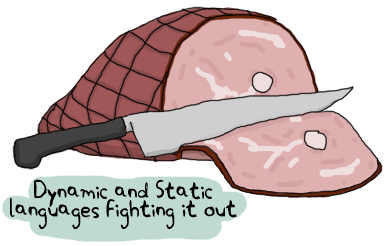
\includegraphics[width=0.4\textwidth]{ham.png}
\end{figure} 
Одно из классических мест трения между сторонниками статической и динамической типизации связано с безопасностью програмного обеспечения.
Часто насаждается идея, что хорошая статическая система типов, за исполнением которой с усердием следят компиляторы, будет ловить большинство ошибок ещё до того как код будет исполнен.
Поэтому языки со статической типизацией считаются более надёжными, чем их динамические собратья.
Хотя для многих динамических языков это действительно так, но к Erlang это относится не в полной мере, и его послужной список это подтверждает.
Лучшим примером служит степень готовности к обслуживанию (availability) \emph{девять девяток} (99.9999999\%), которая обеспечивается на свитчах \href{http://www.erlang.se/publications/Ulf_Wiger.pdf}{Ericsson AXD 301 ATM}.
Количество строк Erlang\--кода для этих устройств \--- свыше 1 миллиона.
Обратите внимание, что это не показатель того, что ни одна из компонент системы, написанной на Erlang, не давала сбой.
Это означает, что свитч как единая система был готов к работе 99.9999999\% времени, включая запланированные перерывы.
Отчасти это вызвано тем, что Erlang построен на идее, что сбой в одной из компонент не должен влиять на всю систему.
Учитываются ошибки, которые делает программист, сбои оборудования или сети.
Язык включает возможности, которые позволяют распределять программы на различные узлы, обрабатывать непредвиденные ошибки и \emph{никогда} не останавливаться.

Короче говоря, в то время как большинство языков и систем типов стараются избавить программы от ошибок, Erlang использует стратегию, согласно которой считается, что ошибки в любом случае будут появляться, и старается эти случаи предотвратить.
Динамическая система типов в Erlang не является преградой для надёжности и безопасности программ.
Звучит это всё как речи проповедника, но в последующих главах вы увидите как это происходит.\\
\colorbox{lgray}
{
    \begin{minipage}{\linewidth}
\textbf{Замечание:} динамическая типизация была избрана исторически по простой причине.
Люди, которые реализовывали Erlang, в большинстве своём имели опыт программирования на языках с динамической типизацией, и поэтому самым естественным выбором для них было сделать Erlang динамическим.
    \end{minipage}
}

Кроме того, Erlang \--- язык с сильной типизацией.
Языки со слабой типизацией производят неявные преобразования типов между термами.
Если бы Erlang был языком со слабой типизацией, то мы, вероятно, могли бы исполнить операцию \ops{6 = 5 + ``1''}, тогда как в действительности будет выброшено исключение, которое сообщает о неверных аргументах:
\begin{lstlisting}[style=erlang]
1> 6 + "1".
** exception error: bad argument in an arithmetic expression
    in operator  +/2
        called as 6 + "1"
\end{lstlisting}

Конечно же, есть моменты, когда вам бы хотелось преобразовать один вид данных в другой.
Например, привести обычный строковый тип к битовым строкам на время хранения, или целое привести к числу с плавающей запятой.
Стандартная библиотека Erlang предоставляет для этого множество функций.
\section{Преобразование типов}
Как и многие языки, Erlang меняет тип терма путём приведения его к другому типу.
Это происходит с применением встроенных функций, поскольку многие преобразования невозможно реализовать на чистом Erlang.
Каждая такая функция принимает форму <тип>\_to\_<тип> и находится в модуле \ops{erlang}.
Вот некоторые из них:
\begin{lstlisting}[style=erlang]
1> erlang:list_to_integer("54").
54
2> erlang:integer_to_list(54).
"54"
3> erlang:list_to_integer("54.32").
** exception error: bad argument
    in function  list_to_integer/1
        called as list_to_integer("54.32")
4> erlang:list_to_float("54.32").
54.32
5> erlang:atom_to_list(true).
"true"
6> erlang:list_to_bitstring("hi there").
<<"hi there">>
7> erlang:bitstring_to_list(<<"hi there">>).
"hi there"
\end{lstlisting}

И так далее.
Здесь мы натыкаемся на особенность языка: так как используется схема <тип>\_to\_<тип>, то при добавлении нового типа в язык, приходится добавлять множество встроенных функций!
Вот их полный список:
\ops{atom\_to\_binary/2, atom\_to\_list/1, binary\_to\_atom/2}\\
\ops{binary\_to\_existing\_atom/2, binary\_to\_list/1,}\\
\ops{bitstring\_to\_list/1, binary\_to\_term/1, float\_to\_list/1,}\\
\ops{fun\_to\_list/1, integer\_to\_list/1, integer\_to\_list/2,}\\
\ops{iolist\_to\_binary/1, iolist\_to\_atom/1, list\_to\_atom/1,}\\
\ops{list\_to\_binary/1, list\_to\_bitstring/1,}\\
\ops{list\_to\_existing\_atom/1, list\_to\_float/1, list\_to\_integer/2,}\\
\ops{list\_to\_pid/1, list\_to\_tuple/1, pid\_to\_list/1,}\\
\ops{port\_to\_list/1, ref\_to\_list/1, term\_to\_binary/1,}\\
\ops{term\_to\_binary/2 и tuple\_to\_list/1.}

Многовато функций.
Большинство из них, если не все, мы увидим в этой книге.
Впрочем, все они нам вряд ли понадобятся.
\section{Охранять тип данных}
Базовые типы Erlang просто заметить: у кортежей есть фигурные скобки, у списков \--- квадратные, строки заключены в двойные кавычки и т.д.
Поэтому определённый тип данных можно использовать в сопоставлении с образцом: функция \ops{head/1}, которая принимает в качестве аргумента список, может принимать списки потому, что для других типов не сработало бы сопоставление (\ops{[H|\_]}).
\begin{figure}[h!]
    \centering
    
\includegraphics[width=0.3\textwidth]{my-name-is.png}
\end{figure} 

Тем не менее, у нас уже возникали проблемы с числовыми значениями, для которых мы не могли задавать диапазоны.
Для решения этой проблемы мы использовали стражи в функциях, которые были связаны с температурой, водительским возрастом и т.д.
Перед нами встаёт ещё одно препятствие.
Как нам записать страж, который применил бы сопоставление с образцом к данным лишь одного определённого типа, такого как числа, атомы или битовые строки?

Для решения этой задачи существуют функции.
Они принимают один аргумент и возвращают истину, если тип верный и ложь в противоположном случае.
Они \--- часть группы из нескольких функций, которые допускаются в охранных выражениях и называются <<встроенными функциями для тестирования типов>>:
\begin{lstlisting}[style=erlang]
is_atom/1           is_binary/1        
is_bitstring/1      is_boolean/1        is_builtin/3       
is_float/1          is_function/1       is_function/2      
is_integer/1        is_list/1           is_number/1        
is_pid/1            is_port/1           is_record/2        
is_record/3         is_reference/1      is_tuple/1        
\end{lstlisting}

Их можно использовать так же как и любое другое охранное выражение, в любом месте, где допускается охранное выражение.
Вы, вероятно, задаёте себе вопрос: почему функция просто не возвращает тип терма, который ей передали (что\--то вроде \ops{type\_of(X) -> Type}).
Ответ довольно прост.
Erlang концентрируется на программировании для правильных случаев: вы составляете программу только для событий, которые точно должно произойти, для тех событий, которые вы ожидаете.
Всё прочее должно как можно раньше вызвать ошибку.
Может быть это покажется абсурдом, но объяснения, которые вы получите в главе \ref{errors-and-exceptions}, я надеюсь, прояснят ситуацию.
А пока что просто поверьте мне на слово.\\
\colorbox{lgray}
{
    \begin{minipage}{\linewidth}
\textbf{Замечание:} встроенные функции определения типа более чем на половину состоят из инструкций, которые можно использовать в охранных выражениях.
Остальные функции также являются встроенными, но не относятся к функциям определения типов.
Среди них: \ops{abs(Number), bit\_size(Bitstring), byte\_size(Bitstring),}
\ops{element(N, Tuple), float(Term), hd(List), length(List),}
\ops{node(), node(Pid|Ref|Port), round(Number), self(),}
\ops{size(Tuple|Bitstring), tl(List), trunc(Number), tuple\_size(Tuple).}\\
Функции \ops{node/1} и \ops{self/0} принадлежат к распределённым средствам Erlang и разделу процессов/акторов.
Вскоре мы будем их использовать, но до той поры нам нужно изучить много других тем.
    \end{minipage}
}

Может показаться, что структуры данных в Erlang относительно ограничены, но списков и кортежей обычно достаточно для создания других более сложных структур.
Например, узел двоичного дерева можно представить как \ops{\{node, Value, Left, Right\}}, где \emph{Left} и \emph{Right} это или узлы, одинаковые по структуре, или пустые кортежи.
Я мог бы представить себя в таком виде:
\begin{lstlisting}[style=erlang]
{person, {name, <<"Fred T-H">>},
    {qualities, ["handsome", "smart", "honest", "objective"]},
    {faults, ["liar"]},
    {skills, ["programming", "bass guitar", "underwater breakdancing"]}}.
\end{lstlisting}

Этот пример показывает, что мы можем получить сложные структуры данных путём вложения списка в кортежи, заполнения их данными, и создания функций, которые будут работать над этой структурой.\\
\colorbox{lgray}
{
    \begin{minipage}{\linewidth}
\textbf{Дополнение:}
в релизе R13B04 появилась встроенная функция \ops{binary\_to\_term/2}, которая позволяет десериализовать данные так же, как это делает \ops{binary\_to\_term/1}, с тем лишь отличием, что вторым аргументом передаётся список опций.
Если передать опцию \ops{[safe]}, то двоичные данные не будут декодированы, если они содержат неизвестные атомы или \ref{higher-order-functions}~анонимные функции, которые могут привести к исчерпанию памяти.
    \end{minipage}
}
\section{Для подсевших на типы}
\label{for-type-junkies}
Этот раздел предназначен для программистов, которые не могут жить без статических систем типов по той или иной причине.
Он содержит слегка усложнённую теорию, которая не всем будет ясна.
Я кратко опишу инструменты, которые используются для статического анализа типов в Erlang, определения специализированных типов, и то, как всё это позволяет получить более безопасный код.
Эти инструменты будут описаны в книге намного позже, потому как они совсем не обязательны для разработки надёжных программ на Erlang.
Так как мы будем рассматривать их позже, я дам лишь основную информацию об их установке, запуске и т.д.
Повторюсь: этот раздел предназначен для тех, кто действительно не может жить без развитых систем типов.
\begin{figure}[h!]
    \centering
    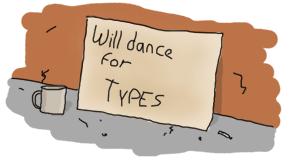
\includegraphics[width=0.4\textwidth]{type-dance.png}
\end{figure} 

На протяжении нескольких лет предпринимались попытки построения системы типов поверх Erlang.
Одна из таких попыток случилась в 1997 году под руководством Simon Marlow, одного из ведущих разработчиков Glasgow Haskell Compiler и Philip Wadler, который работал над проектированием Haskell и внёс свою лепту в теорию, которая лежит в основе монад (\href{http://www.haskell.org/~simonmar/papers/erltc.pdf}{вы можете прочитать документ} посвящённый упомянутой системе типов).
Joe Armstrong позже \href{http://www.cs.chalmers.se/Cs/Grundutb/Kurser/ppxt/HT2007/general/languages/armstrong-erlang\_history.pdf}{прокомментировал документ}:\\
\colorbox{lgray}
{
    \begin{minipage}{\linewidth}
Однажды мне позвонил Фил и заявил, что а) Erlang необходима система типов, б) он написал непольшой прототип такой системы и в) у него есть возможность взять годичный отпуск, в течение которого он собирался написать систему типов для Erlang, и спрашивал: <<заинтересованы ли мы в этом?>>.
Я ответил: <<Да.>>\\
Phil Wadler и Simon Marlow работали над системой типов больше года, и результаты были опубликованы в [20].
Результаты немного разочаровывали.
Начнём с того, что на соответствие типов можно было проверять лишь подмножество языка, большим упущением было отсутствие типизированных процессов и отсутствие проверки типов для сообщений, передаваемых между процессами.
    \end{minipage}
}

Процессы и сообщения относятся к основным средствам Erlang.
Может быть именно поэтому система так никогда и не была добавлена в язык.
Были и другие неудачные попытки типизировать Erlang.
В результате усилий проекта HiPE (попытка увеличить производительность Erlang) появился Dialyzer, инструмент статического анализа, который используется до сих пор.
Он имеет свой собственный механизм вывода типов (type inference).

Система типов, которая в нём используется, основана на успешных типизациях (success typings) \--- концепции, которая отличается от системы типов Hindley\--Milner или мягкой типизации (soft\--typing).
Концепция успешной типизации проста: метод определение типов не будет пытаться найти точный тип каждого выражения, но он будет гарантировать, что выведенные им типы точны, и что ошибки типов, которые он находит, действительно являются ошибками.

В качестве примера лучше всего привести реализацию функции \ops{and}, которая обычно принимает два булевых значения и возвращает 'true', если оба параметра истинны, иначе возвращается 'false'.
В системе типов Haskell это можно записать как \ops{and :: bool -> bool -> bool}.
Если бы нужно было реализовать функцию \ops{and} на Erlang, то это можно было бы сделать следующим образом:
\begin{lstlisting}[style=erlang]
and(false, _) -> false;
and(_, false) -> false;
and(true,true) -> true.
\end{lstlisting}

Применяя метод успешной типизации, выведенный тип был бы \ops{and(\_,\_) -> bool()}, где \_ означает 'что угодно'.
Это происходит по простой причине: когда запускается программа на Erlang и вызывается эта функция с аргументами \ops{false} и \ops{42}, будет возвращён результат 'false'.
Использование шаблона подстановки \ops{\strut\_} в сопоставлении с образцом привело к тому, что для работы функции достаточно передать хотя бы один аргумент, который равен 'false'.
У системы типов ML случился бы припадок (а у её пользователей сердечный приступ), если бы вы вызвали функцию таким образом.
Но не у Erlang.
В этом появится больше смысла, если вы решите прочитать документ про \href{http://www.it.uu.se/research/group/hipe/papers/succ\_types.pdf}{реализацию успешной типизации}, в котором объясняется логика, которая стоит за таким поведением.
Я призываю любого наркомана, зависимого от типов, прочитать эту статью.
Она представляет собой интересное и полезное описание реализации метода.

Подробности об определениях типов и аннотациях функций описаны в Предложении об Улучшении Erlang №8 (\href{http://www.erlang.org/eeps/eep-0008.html}{EEP8}).
Если вас заинтересовало использование успешной типизации в Erlang, взгляните на \href{http://user.it.uu.se/~tobiasl/publications/typer.pdf}{приложение TypEr} и Dialyzer.
Оба входят в стандартный дистрибутив.
Чтобы ими воспользоваться, введите \ops{\$ typer --help} и \ops{\$ dialyzer --help} (для Windows команды \ops{typer.exe --help} и \ops{dialyzer --help}, если они доступны из текущей директории).

TypEr используется для создания аннотаций типов для функций.
Запуск TypEr для этой маленькой \href{http://learnyousomeerlang.com/static/erlang/fifo.erl}{реализации FIFO очереди}, генерирует следующее описание типов:
\begin{lstlisting}[style=erlang]
%% File: fifo.erl
%% --------------
-spec new() -> {'fifo',[],[]}.
-spec push({'fifo',_,_},_) -> {'fifo',nonempty_maybe_improper_list(),_}.
-spec pop({'fifo',_,maybe_improper_list()}) -> {_,{'fifo',_,_}}.
-spec empty({'fifo',_,_}) -> bool().
\end{lstlisting}

Что, в целом, верно.
Неправильные списки лучше не использовать, так как \ops{lists:reverse/1} их не поддерживает, а кто\--либо, минуя интерфейс модуля, сможет всё\--таки протолкнуть такой список.
В этом случае функции \ops{push/2} и \ops{pop/2} всё же успешно отработают несколько вызовов, перед тем как будет выброшено исключение.
Это говорит нам, что необходимо добавить стражи, либо вручную оптимизировать наши определения типов.
Предположим, мы добавили в модуль сигнатуру \ops{-spec push(\{fifo,list(),list()\},\_) -> \{fifo,nonempty\_list(),list()\}.} и функцию, которая передаёт неправильный список для \ops{push/2}.
При сканировании Dialyzer\--ом (который проверяет типы на соответствие), будет выведено сообщение об ошибке <<The call fifo:push({fifo,[1|2],[]},3) breaks the contract '<Type definition here>\'>>.
\begin{figure}[h!]
    \centering
    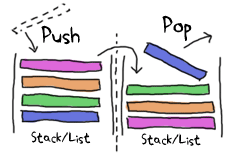
\includegraphics[width=0.4\textwidth]{fifo.png}
\end{figure} 

Dialyzer будет сообщать об ошибках лишь в том случае, когда код будет ломать другой код, и эти сообщения обычно будут оказываться верными (также он будет сообщать и о других проблемах, например о ветках, до которых никогда не дойдёт исполнение или об общем рассогласовании).
При помощи Dialyzer\--а также можно анализировать полиморфные типы данных.
Функцию \ops{hd()} можно описать при помощи \ops{-spec([A]) -> A.} и корректно проанализировать, впрочем программисты на Erlang редко используют этот синтаксис описания типов.\\
\colorbox{lorange}
{
    \begin{minipage}{\linewidth}
        \textbf{Не забывайтесь:}\\
Dialyzer и TypEr не обрабатывают типовые классы с конструкторами, типы первого порядка и рекурсивные типы.
Типы в Erlang \--- это лишь аннотация, которая не влияет и не ограничивает компиляцию, кроме случаев, когда вы сами накладываете эти ограничения.
Программа проверки типов никогда не сообщит вам, что в приложении, которое исполняется прямо сейчас (или исполняется уже на протяжении двух лет), есть ошибка типов, которая никак себя не проявляет во время исполнения (впрочем, код с ошибками может корректно исполняться\ldots)\\
Было бы весьма интересно иметь возможность создания рекурсивных типов, но они вряд ли когда\--нибудь появятся для текущей формы TypEr и Dialyzer (объяснение содержит статья, указанная выше).
Лучшее, что можно сделать на текущий момент, это симулировать рекурсивные типы при помощи нескольких уровней вложенности, добавленных вручную.\\
Конечно же, нельзя это называть всеобъемлющей системой типов, сравнимой со строгостью и мощью систем, которые предлагают Scala, Haskell или OCaml.
Её сообщения о предупреждениях и ошибках обычно слегка запутаны и не всегда ясны пользователю.
Тем не менее, это решение предлагает очень неплохой компромисс, если вы просто не можете существовать в мире динамического языка или жаждете дополнительной надёжности.
Относитесь к этому как к инструменту в вашем арсенале, не более.
    \end{minipage}
}
\colorbox{lgray}
{
    \begin{minipage}{\linewidth}
\textbf{Дополнение:}\\
Начиная с версии R13B04, в Dialyzer была добавлена экспериментальная возможность работы с рекурсивными типами.
Этот факт делает предыдущий раздел отчасти неверным.
Стыд мне и позор.\\
Также заметьте, что \href{http://erlang.org/doc/reference\_manual/typespec.html}{документация типов стала официальной} (хотя она и сможет в будущем измениться) и более полной, чем в EEP8.
    \end{minipage}
}
